\clearpage % clearpage places the content underneath on to a new page

\section{A Guide to Writing and Using \LaTeX} \label{sec:UsingLaTeXGuide}
The following sections provide some direction on how to typeset with \LaTeX. Word processing applications utilising  a ``What You See Is What You Get'' (WYSIWYG) type user interface (``Word'' / ``Writer'') are designed for general purpose use. Such applications are not designed for the creation of professional documents and reports requiring high levels of precision to ensure all elements from the individual characters of a word to the placement of tables and figures are presented as they should be. 

A key advantage of \latex is the decoupling of the content from the presentation. This inherently allows one to focus on what is of greatest importance, the content. With \latex one can write code akin to the HTML and CSS relation of decoupling content from presentation, the result of which can be compiled into a professionally typeset document, be it a report, cv, presentation or poster for example. When one needs to develop a professional and structured document then the ``You Asked For It You Got It'' (YAFIYGI) route that many in computing, maths and physics embrace is the generally preferred solution toward achieving a timely and high quality output. 

\subsection{Adding Figures (Images / Graphics) to the Report}

Add an image file to the ``\textbf{images}'' folder. Then replicate the code in this subsection, which generates Figure \ref{fig:samplepngImage}. One should then modify the \textbf{label}, \textbf{caption} and \textbf{image file name} to suit. The size of the image is scaled relative to the content width of the page, Figure \ref{fig:samplepngImage} in this case is set to 40\% (0.40) of the content width. 

\begin{figure}[H]
\begin{center}
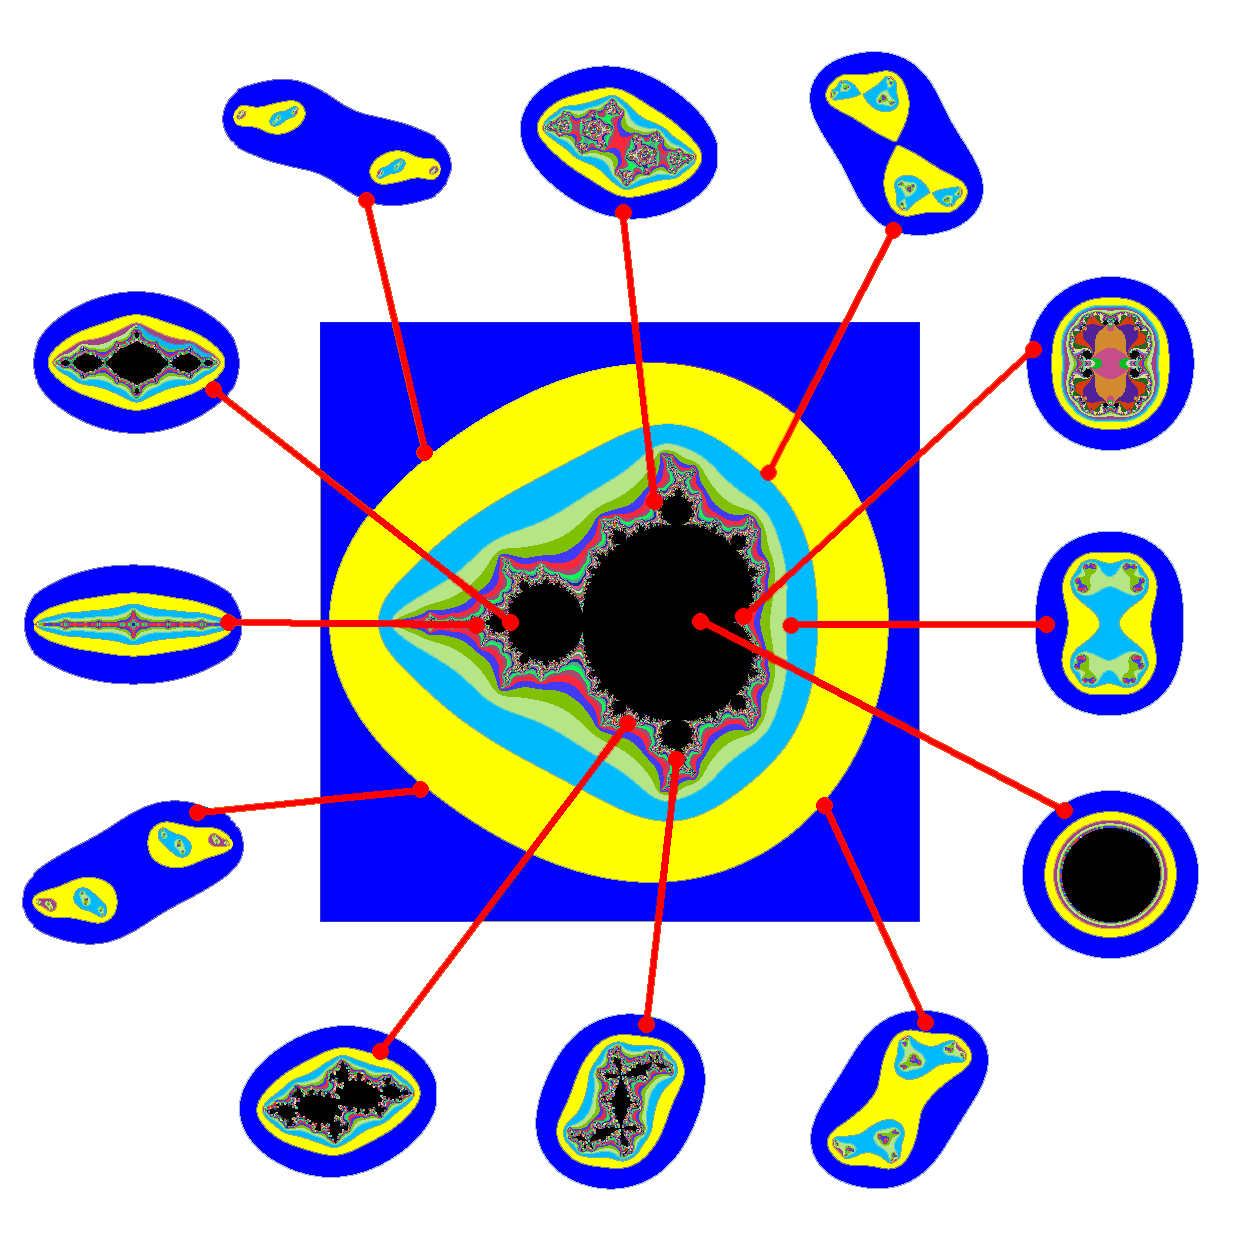
\includegraphics[width=.40\linewidth]{samplepng.png}
\caption{Caption for Bitmap Image (MSet Fractal and Associated JSets)} \label{fig:samplepngImage}
\end{center}
\end{figure}
\subsubsection{More on Figures \& use of Vector Graphics for High Quality Diagrams}
One can insert graphic elements using \latex in a number of ways. Vector based imagery such as diagrams saved to the pdf format may use the \emph{\textbackslash includegraphics} command with the optional \emph{viewport} attribute to specify a precise area of the graphic to be included. 

When inserting a Figure (Figure~\ref{fig:VectorGraphicElementPDF}) one uses the \emph{\textbackslash begin\{figure\}} and \emph{\textbackslash end\{figure\}} commands. The image presented is a vector graphic in the form of a pdf file. When working with such files it is usually necessary to include the optional \emph{viewport} attribute to designate the specific area in which to focus. The first pair of coordinates (x~\&~y) designate the pixel location of the lower left corner. The second pair identify the upper right hand corner. Modification of these coordinates allows one to focus in upon a particular area of interest within the vector image. 

The optional attribute [H] when beginning a Figure inserts the graphic element at the specified location. Other options such as [htb] (here, top, bottom) will place the graphic in the most suitable place that \latex can find. This however can have a negative impact on memory allocation if a large number of images exist, therein preventing compilation.


\begin{figure}[H]
\centering
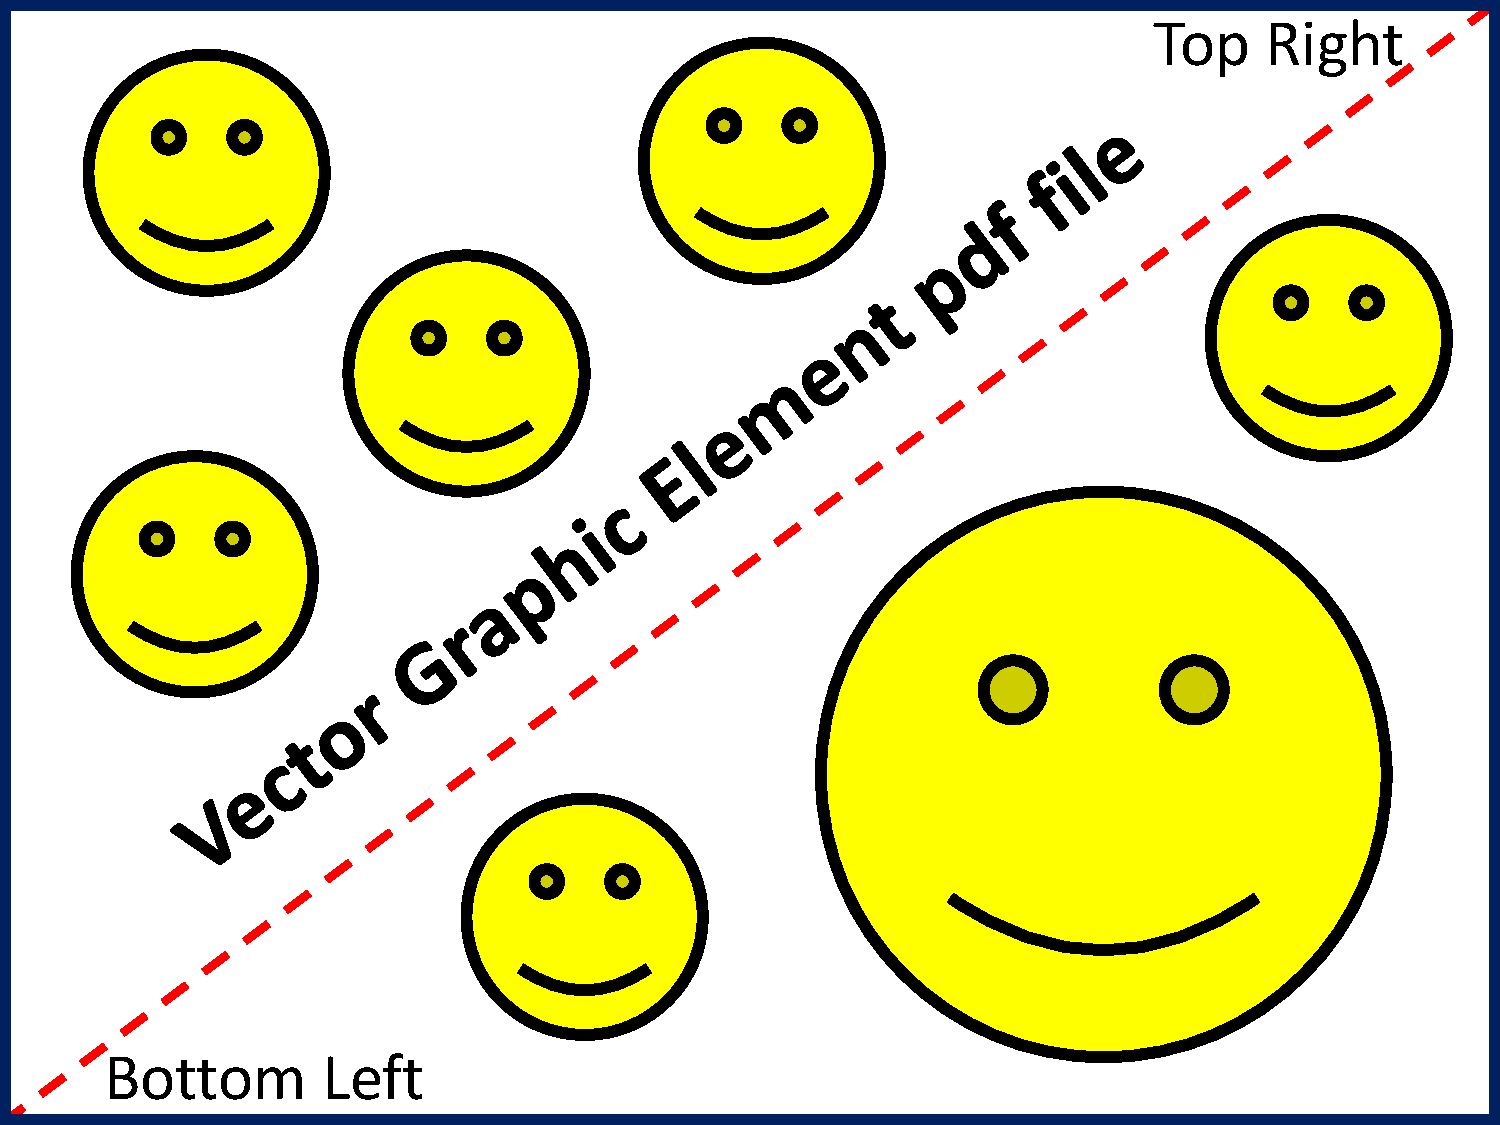
\includegraphics[width=.4\linewidth]{VectorGraphicElementPDF.pdf}
\caption{Vector Graphic - pdf of a PowerPoint Slide}
\label{fig:VectorGraphicElementPDF}
\end{figure}

One may use the \emph{minipage} command when inserting two figures to span across the page. This allows for the subdividing of the page into a number of columns of specified width. Figure~\ref{fig:Example1} \&~\ref{fig:Example2} demonstrate how one may zoom in / focus on a particular section of a graphic by altering the coordinates of the \emph{viewport}. 

\begin{figure}[H]
\begin{minipage}[t]{7.4cm}
\begin{center}
\includegraphics*[viewport= 20 20 600 440, width=.8\linewidth]{VectorGraphicElementPDF.pdf}
\caption{Viewport = 20 20 600 440}
\label{fig:Example1}
\end{center}
\end{minipage}
\hfill
\begin{minipage}[t]{7.4cm}
\begin{center}
\includegraphics*[viewport= 220 200 400 330, width=.8\linewidth]{VectorGraphicElementPDF.pdf}
\caption{Viewport = 220 200 400 330}
\label{fig:Example2}
\end{center}
\end{minipage}
\end{figure}

The key advantage to using vector imagery for diagrammatic and textual content is that such imagery contains embedded instruction on what is to be drawn, therefore it can scale to any size without loss of image quality. This contrasts with a bitmap or raster image which results in a matrix / array of pixel values. If saving a screenshot then  .png is preferable over a .jpg which is a lossy file format yielding many artefacts with image content which transitions rapidly, such as from text or a line to a background.

\subsection{Adding a Table with the Tabular Environment}
Replicate the code in this subsection, which generates Table~\ref{tab:TableExample}. One should modify the \textbf{label}, \textbf{caption} and \textbf{content} of the table to suit. 
\begin{table}[H]
\caption{Place a Caption for the Table Here}\label{tab:TableExample}
\centering
\small
\begin{tabular}{lllp{5cm}}
\toprule \textbf{Heading 1}& \textbf{Heading 2}&\textbf{Heading 3}&\textbf{Heading 4}\\
\midrule
Cell A1 & Cell B2 & Cell C3 & Cell D4\\
Cell E1 & Cell F2 & Cell G3 & Justified text with a defined column size of 5cm\\
\bottomrule
\end{tabular}
\end{table}

The cells in Table~\ref{tab:TableExample} displays three columns of left-aligned and one column of justified data. Cell contents can be aligned to the left (l), right (r), center (c) or paragraph (p). Vertical bars may sometimes be seen in tables but these generally look unprofessional. The Booktabs package \cite{online:Fear2005BookTabs} allows for the creation of professional looking tables as shown in the example.  The use of \emph{\textbackslash toprule}, \emph{\textbackslash midrule} and \emph{\textbackslash bottomrule} commands provided by the package allow for rules of varying thickness and spacing. Data elements (cells / columns) within a table are separated using the ampersand (\&). Completion of a row ends with a double backslash (\textbackslash\textbackslash). Both tables and figures need a caption and a label.

\subsection{Citing References to other Articles / Publications}
In this report references are stored in a database with the file name ``{\tt references.bib}'', this contains a list of articles, proceedings, books, thesis and online information sources. Each type of publication has a number of required fields such as a unique identifier, author and title. To cite a reference within the main body text one must use the \emph{\textbackslash cite} command as per the following examples. Donald Knuth \cite{book:knuth_1973} for example is well known for his work on the Art of Computer Programming. The SETI@Home project \cite{online:berkeleyBOINC} is an example of a webpage citation. One can also work with articles \cite{art:Russell:1978:Cray1}, MSc Thesis \cite{msc:Shannon:1940}, PhD Thesis \cite{phd:Sutherland:1963} or articles within conference proceedings \cite{proc:Ewald:1978:HPG}. Dr. Doolan \cite{online:Doolan:2016:AcademicResources} has provided an online list of resources that may be useful for undertaking literature reviews along with a number of useful \latex tools. 

\subsubsection{References within a Reference Highlighting Pages or other Elements}
To refer to a particular page, section, chapter, equation or other element of a large document add the corresponding information within square brackets right after the \emph{\textbackslash cite} command, such as \emph{\textbackslash cite[p. 2]$\{$online:IEEE-ReferenceGuide:2018$\}$}. Further information is available from the ``IEEE Reference Guide'' \cite[p.3]{online:IEEE-ReferenceGuide:2018}, located in section I.B \cite[Sec I.B]{online:IEEE-ReferenceGuide:2018}. Table~\ref{tab:ReferenceExamples} illustrates a number of common elements one may refer to within a citation, in this case pages or elements of reference ``42'' \cite[Ch. 27]{book:Adams:1979}.

\begin{table}[H]
\caption{Examples of References within a Reference}\label{tab:ReferenceExamples}
\centering
\small
\begin{tabular}{ll}
\toprule \textbf{Reference Type}& \textbf{Presentation Format}\\
\midrule
A Single Page & [42, p. 8] \\
Range of Pages & [42, pp. 4-8] \\
Figure & [42, Fig. 8] \\
Table & [42, Tab. 4] \\
Appendix & [42, Appendix. F] \\
Specific Section & [42, Sec. 4.8] \\
Chapter and Pages & [42, Ch. 4 pp 42-64] \\
An Algorithm & [42, Alg. 4] \\
An Equation & [42, eq. (4)] \\
\bottomrule
\end{tabular}
\end{table}

\subsubsection{Referencing Style}
Quite a number of Universities use the ``Harvard'' referencing style, this makes use of the author name and date in the body text of the report to make a citation. The references generally found at the end of the report are sorted by author name. Several subject disciplines regularly use the Harvard format such as the arts, humanities and business. This is fitting with a more discursive narrative common amongst those subject areas. 

It is always useful to check the University Referencing Style Guide for your institution. You will find that the University Library provides detailed information and examples on how to reference. Many University Style Guides may suggest Harvard as the institutional standard, however they may also stipulate the use of the most appropriate style for the discipline. It is always useful to check the University Referencing Style Guide for your institution. The IEEE Referencing Style in this template is regularly used in Computing.      

In Computing it is far more common to see citations in the body text represented as a number within square brackets. The associated references are listed in the order they appear within the body text, preceded with the associated reference number. An advantage with this referencing style is far less real-estate being occupied by the citation. 

\subsubsection{Referencing Another Element of the Report}
To refer to another part of the document one must use a combination of the \emph{\textbackslash ref} and \emph{\textbackslash label} commands. The label is a unique identifier, therefore when working with large documents it helps to give references meaningful names. Examples of this includes prefixing Table references with \emph{tab:}, figures with \emph{fig:}, chapters with \emph{ch:}. The tilde ($\sim$) known as a ``tie'' in \latex is used to ensure that a reference remains as a single unified object. All instances of \emph{\textbackslash ref} should be preceded with the tilde. Section~\ref{sec:WorkWithMath} refers to ``Working with Mathematics'' identified with \emph{\textbackslash label$\{$sec:WorkWithMath$\}$} right after the section heading and referred to here via the instruction \emph{Section$\sim$\textbackslash ref$\{$sec:WorkWithMath$\}$}. 

\subsection{Creating Numeric and Bulleted Lists}
Replicate the code in this subsection to create numbered or bulleted lists. As can be seen in the example below one can create different levels of list elements if necessary. Its best to limit the use of lists and focus more on paragraphs of text to convey the narrative of a report. Lists can sometimes be useful emphasise key elements. 

{\setstretch{0.5}% Reduces line spacing to compact the list items
\begin{enumerate}
\item First element of a numbered list
\item Second element of a numbered list
\end{enumerate}
\begin{itemize}
\item First element of a bulleted list
\item Second element of a bulleted list
    \begin{itemize}
    \item First nested element of a bulleted list
    \item Second nested element of a bulleted list
    \end{itemize}
\end{itemize}
} % Closing Parenthesis  with respect to the use of \singlespacing for the display of the list elements

\subsection{Working with Mathematics}\label{sec:WorkWithMath}
The power of \latex in typesetting mathematical formula is one of its key strengths. In the realm of fractals the Mandelbrot Set or MSet defined as: $Z_{n+1} =
Z_{n}^2 + C$, is an example of some math included within the body text of a paragraph. Matrix Multiplication is typically regarded as an $O(n^3)$
operation. One may use the \emph{equation} environment for more complex mathematical formula that should standout. For example the product  $C$ of two matrices $A \in M_{n,m}(R)$ and $B \in
M_{m,p}(R)$ may be defined as:

\begin{equation}
(A \times B)_{ij} = \sum_{k=0} ^{m-1} a_{ik}b_{kj},~
i=0,...,n-1,~j=0,...,p-1.
\end{equation}

The sizes of the matrices must satisfy $(n \times m)(m \times p) = (n \times p)$. Matrix multiplication is an associative process thereby $a\cdot(b \cdot c) = (a \cdot b) \cdot c$. Essentially to find the value of a particular cell $C_{i,j}$ it is necessary to multiply row $i$ of the matrix $A$ with column $j$ of matrix $B$ summing all the multiplications.

\subsection{Using the Correct Quotes}
To surround a piece of text with double quotes one must place two single quotes on either side of the text. The double quote on the left is created using two left quotes (\lq) this is located just above the \emph{tab} key on the keyboard. The right hand double quote is created using two right hand quotes via (\rq) located just above and to the left of the right shift key. A properly formatted quotation should look like ``This is a quotation''. Notice how the direction of the quotes are opposite to one another. A larger example using the \emph{\textbackslash Huge} font size option, is presented below so the quotes can be clearly seen.
\begin{center}
\Huge{``This is a quotation''}
\end{center}
When including text from another source be it online, a book, another report, thesis or other, then it should be surrounded with quotes and a reference to the source provided. 

\subsection{Inserting an Algorithm}
The \emph{algorithm2e} environment \cite{online:Fiorio2016algorithm2e} may be used to generate algorithms (Algorithm~\ref{alg:SampleAlgorithm}). If no algorithms are used within the document then comment out \emph{\textbackslash listofalgorithms } in the file ``{\tt main.tex}'' to remove the list of algorithms heading.

\begin{algorithm}
%\dontprintsemicolon
\While{(RANK $<$ COMPSIZE)}{
    \If{(RANK == MASTER)}{
        generate random value \;
        \For{(each item K)}{
            get result \;
        }
    }
}
\caption{A Sample Algorithm in the Domain of Parallel Computing} \label{alg:SampleAlgorithm}
\end{algorithm}

\subsection{Widows and Orphans Anomalies to Avoid when Writing}
These anomalies can occur at the paragraph and page level. A paragraph where a single word or two flows over on to a new line is inherently wasting valuable space on the page. It is thereby worthwhile to review and rephrase the paragraph to avoid such instances \textcolor{red}{occurring.}  

The paragraph above is a good example of such wasted space, take note of the last word of the paragraph ``occouring'', in essence it is positioned all alone, away from all the other words compromising the unit paragraph. 

Another example is where the starting line of a paragraph begins at the end of a page, with the bulk of the paragraph existing on the next page. Making use of \emph{\textbackslash clearpage} can often help, to push the entire paragraph on to the next page. Likewise the last sentence of a paragraph may run over onto the next page. One should again review and rephrase the paragraph as necessary to avoid this, therein maintaining the structural integrity and cohesiveness of the paragraph as a single clearly defined unit. 

\subsection{What is a Paragraph}
All too often one sees paragraphs comprising of a single sentence, comprising a line or two. Such is inherently not a paragraph. A paragraph should ideally comprise around half a dozen plus sentences, focused on are particular topic of discussion. Often the starting sentence of the paragraph introduces the concept, while the last sentence concludes the discussion put forth. Hence a paragraph should be a cohesive unit of narrative unto itself. This paragraph, not withstanding this sentence, started out by outlining a common problem with paragraphs, then explained the expected structure and concluded that it should be a standalone unit of prose. 

\clearpage
\subsection{Conclusion the \latex Advantage}
All professionally written reports should end with a conclusion summing up the main elements of the report, key results obtained and potential future directions. Large reports are generally broken into chapters, each ending with a conclusion which may also lead on to the next chapter. Such large reports would commonly have a conclusion chapter at the end. In the case of a short report for a university assignment a conclusion section at the end such as this would be common to see. 

By making use of \latex one can focus on the content. As one will see by compiling the source code of this document, all the material is laid out without having to spend significant amounts of time focused on the presentation elements. All the presentation elements from headings and section numbering are automatically generated, as are things such as report front matter, table of contents and references to highlight just a few. 

\subsection{\latex Setup and Install on a Local Machine}
The implementation of \latex that is often used is MikTeX (\url{http://miktex.org}). It is typically best to install the complete MiKTeX  system. A complete system comprises of around 40K files. A minimal install will necessitate the installation of packages as needed. One can individually download and integrate packages into a MikTeX system using the ``Package Manager (Admin)'' application. Initially a small installer application must be downloaded and executed. This in-turn downloads the most recent implementation of the MikTeX system. Run the installer again and select the directory of the downloaded package. Mac users can use the MacTeX distribution (\url{http://www.tug.org/mactex/}).

\subsubsection{Front End Editor}
Texmaker (\url{https://www.xm1math.net/texmaker/download.html}) is a very useful free GUI based editor that includes a built in document viewer. TeXnicCenter is a free download available at (\url{http://sourceforge.net/projects/texniccenter/}). An alternative is WinEdt a shareware ASCII editor (\url{http://www.winedt.com}). WinEdt can be freely used for a 30 day period, after which one will periodically receive reminders to register the product. WinShell (\url{http://www.winshell.de}) is another option for Windows users. An advantage of WinShell is its in-built BibTeX GUI editor. It also has a useful Table Wizard. TexShop (\url{http://pages.uoregon.edu/koch/texshop/}) is a popular option for Mac users, providing a very easy to use editor. Note the website links in this section were created using the \emph{\textbackslash url} command and included for ease of reference. One should ideally include such content as references.  

\clearpage

\subsection{Compiling and Editing on a Local Machine}
{\setstretch{0.75}
\begin{enumerate}
\item Read these instructions ``{\tt main.pdf}'', compare the code in ``{\tt howToGuide.tex}'' to that of the resultant output of Section~\ref{sec:UsingLaTeXGuide} ``A Guide to Writing and Using \LaTeX.'' 
\item Download and install the back-end \latex system and front-end text editor. 
\item Compile ``{\tt main.tex}'' and ``{\tt references.bib}'' to generate the file ``{\tt main.pdf}''.
\begin{enumerate}
\item To achieve this compile with pdfLaTeX, then run BibTeX and compile with pdfLaTeX two further times.
\item It is only necessary to run BibTeX when new citations are added.
\item Two compiles of pdfLaTeX is sufficient to allow for correct reference linkage.
\item If one is simply adding additional content (text / figures / tables) then a single compile of pdfLaTeX is sufficient for testing purposes.
\end{enumerate}
\item Several additional files may now be seen in the root folder of this template, these are generated as part of the compilation process.
\item With a successful compile achieved, start reading through the \latex documents (.tex) to see how the various elements are assembled.
\item Begin editing the document starting with ``{\tt titlepage.tex}'' by entering elements such as Report and Module Titles.
\item When it is necessary to start inserting figures / tables and so forth, copy and paste the \latex code provided and edit the filename, captions, labels and cell content.
\end{enumerate}}

\section{Coursework Assignments a Marathon not a Sprint}
Upon release of a coursework start immediately by firstly fully understanding what is required. Make full use of the time provided, making headway straight away, this will provide positive reinforcement and help propel the work along. A good analogy is that of the ``Gym'' or "DevGym" / ``Development Gym of Learning and Skills'' only by the investment of regular and consistent work, will results be achieved. As Gandalf eloquently puts it ``All we have to decide is what to do with the time that is given us'' \cite{book:Tolkien:1991:FOTR}\cite{online:Jackson:2001:FOTR}. 

Professor Randy Pausch is well known for this work on ``Alice 3D'' and his lectures on ``Time Management'' and ``Fulfilling your Childhood Dreams''. Both of these lectures are well worth watching, Dr. Doolan \cite{online:Doolan:2015:PauschLecture} outlines the main elements of both lectures. Dr. Doolan \cite{online:Doolan:2016:SchwarzeneggerInterview} highlights the key elements of success in the form of Goals, Confidence and Time Management. The post once again summarizes and provides links to the key elements of a video interview with Arnold Schwarzenegger. 

\section{Appendix: Rotated Graphics and Tables}
This additional section, in essence an appendix makes use of the \emph{rotating} package to rotate both figures (Figure~\ref{fig:sidewaysFigure}) and tables (Table~\ref{tab:sidewaysTable}) ninety degrees allowing for large data-sets and illustrations to be clearly presented. The images / figures in this template have been provided courtesy of Dr. Doolan (\url{https://dcdoolan.wordpress.com}). 

\begin{sidewaystable}
\begin{center}
   \begin{tabular}{lllllllll} 
   \toprule
   \textbf{Heading 1} & \textbf{Heading 2}  & \textbf{Heading 3}  & \textbf{Heading 4}  & \textbf{Heading 5}  & \textbf{Heading 6}  & \textbf{Heading 7}  & \textbf{Heading 8}  & \textbf{Heading 9}  \cr
   \midrule
   AAAA & BBBB & CCCC & DDDD & EEEE & FFFF & XXXX & YYYY & ZZZZ \cr 
   AAAA & BBBB & CCCC & DDDD & EEEE & FFFF & XXXX & YYYY & ZZZZ \cr 
   AAAA & BBBB & CCCC & DDDD & EEEE & FFFF & XXXX & YYYY & ZZZZ \cr 
   AAAA & BBBB & CCCC & DDDD & EEEE & FFFF & XXXX & YYYY & ZZZZ \cr 
   AAAA & BBBB & CCCC & DDDD & EEEE & FFFF & XXXX & YYYY & ZZZZ \cr 
   AAAA & BBBB & CCCC & DDDD & EEEE & FFFF & XXXX & YYYY & ZZZZ \cr 
   \bottomrule
   \end{tabular}
\caption[A Short Caption for the Table]{
	A much longer caption that will not be listed in the list of tables page.
}
\label{tab:sidewaysTable}
\end{center}
\end{sidewaystable}

\begin{sidewaysfigure}
\centerline{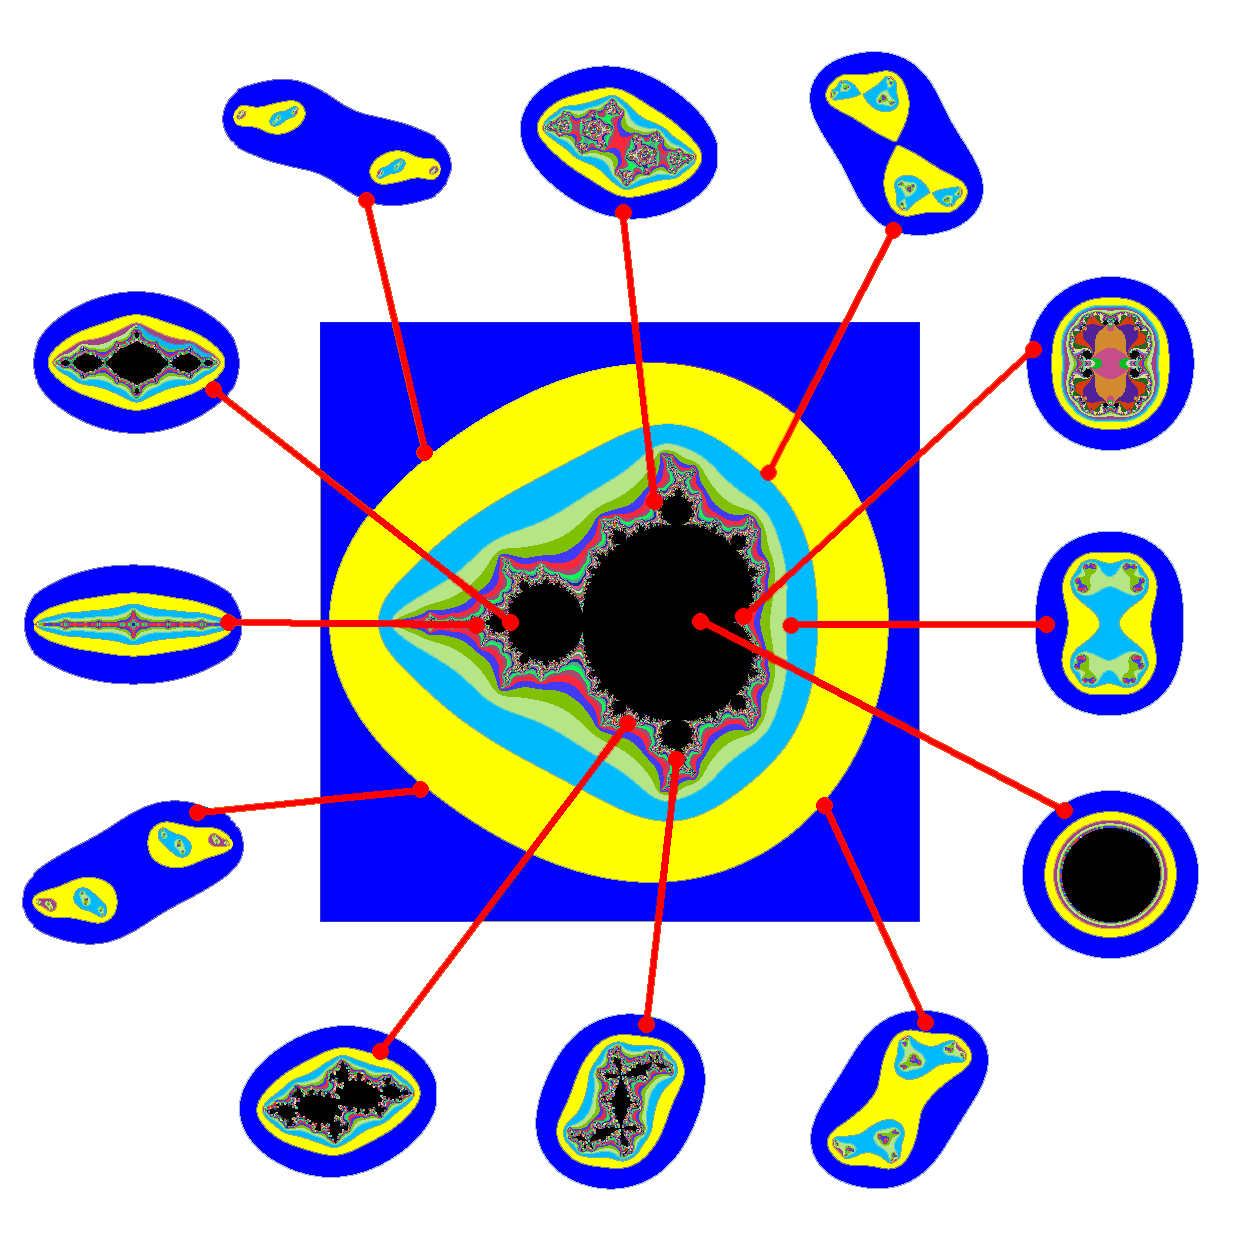
\includegraphics[width=7in]{samplepng.png}}
\caption[A Large Sideways Figure]{
	A much longer caption that will not be listed in the list of figures page (MSet Fractal and Associated JSets).
}
\label{fig:sidewaysFigure}
\end{sidewaysfigure}

